% !TEX root =  ../../thesis.tex

\chapter{Simulation study}
\label{ch : simulation_study}

In this chapter we will share results from the simulation study we performed to check the efficacy of the model selection criteria described in Chapter \ref{ch : model_selection}. We implemented the Bayesian heterogeneity model using the R package R2jags \citep{su_r2jags:_2015} and analyzed the MCMC chains using the R package ggmcmc \citep{marin_ggmcmc:_2016}. For the calculation of marginal likelihood we required the density function of Wishart distribution, which was available in two packages, namely MCMCpack and mixAK. There were inconsistencies in the results from the two implementations and we eventually used mixAK \citep{komarek_mixak:_2015} as the MCMCpack package produced density function value to be $\infty$ in some cases.

\section{Data sets for simulation study}
The data sets we simulated were motivated by the study on predicting Zebu cow's weights in sub Saharan Africa \citep{lesosky_live_2012}. We assumed our response to be the weight of the Zebu cows. The predictors we considered were hypothetical, namely gender of a cattle (Male/Female), birth year of the cattle (1996/1997), age of the cattle at the first measurement and the time at which measurement was taken. The measurements of the cows were done at 10 different equally spaced time intervals. We further added subject specific random intercept and random slope effect to each response so that the repeated measurements for a given cow were correlated. Simultaneously we made sure that these cow specific random effects were mixture distributed. We will refer to the cows as subjects here forth.

\subsection{Description of each data set}
\label{subsec : ds_description}
Our aim was to create data sets differing in number of mixture components for random effects, number of subjects, statistical power to detect the fixed effects, separation of mixture components and number of subjects per component. To analyze the efficacy of model selection criteria under these different scenarios we created multiple data sets. To get a rough idea about the random effects in each of these data sets, we first did a graphical analysis. For this purpose we first regressed the response $\boldsymbol{y}$ on the 3 predictors: age, gender and birth year of cattle using OLS(section \ref{subsec : choice_starting_values}). It is also possible to use linear mixed model for estimating the fixed effects. We then regressed the residuals $y_{ij} - \boldsymbol{x}_{ij}\boldsymbol{\beta}$ on the intercept and time of measurement for every subject separately to obtain a rough estimate $\boldsymbol{\tilde{b}}_i$ of the random effect of subjects. This estimator however overestimates the actual size of the random effects as within subject variance is also included. It is not possible to use Empirical Bayes estimates of the random effects because they may fail to reflect the heterogeneity in the random effects population \citep{verbeke_linear_1996}. Lastly, it is important to note that fitting an incorrect mean structure can lead to a incorrect representation of the random effects distribution as shown in figure \ref{fig : missing_continuous_covariate_randplot}.

\subsubsection{Data set 1: No mixture distribution of random effects}
\label{subsubsec : ds_simple}
The first data set we created was without a mixture of random effects. i.e. $\boldsymbol{b}_i \sim N(0, G)$. In total we generated data of 80 subjects, each having 10 repetitions. Based on the approach mentioned above, a plot of the random effect values for this data set is shown in figure \ref{fig : ds_simple_randplot}.

\subsubsection{Data set 2: 3 well separated components for the mixture of random effects}
\label{subsubsec : ds_3wellsep}
The next data set we created had 3 well separated components forming the mixture distribution of random effects. In total we generated data of 180 subjects, each having 10 repetitions. A plot of the rough estimates of random effect values for this data set is shown in figure \ref{fig : ds_3wellsep_randplot}.

\begin{figure}[!htb]
\centering
	\begin{subfigure}[b]{0.4\textwidth}
		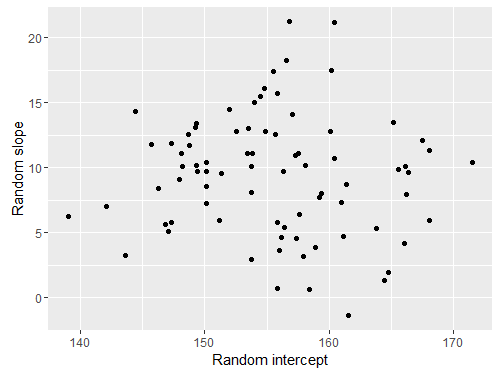
\includegraphics[width=\textwidth]{mainmatter/chapter_5_simulation_study/ds_simple_randplot.png}
       \caption{\label{fig : ds_simple_randplot}Data set 1}
	\end{subfigure}    
	\begin{subfigure}[b]{0.4\textwidth}
		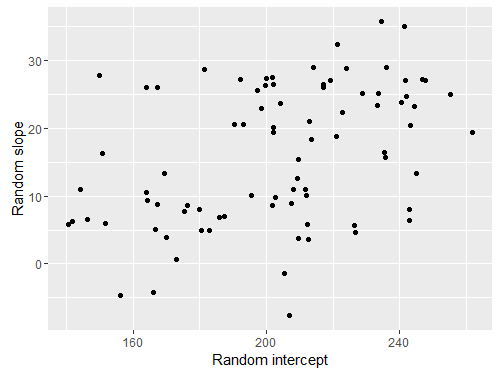
\includegraphics[width=\textwidth]{mainmatter/chapter_5_simulation_study/missing_continuous_covariate_randplot.png}
       \caption{\label{fig : missing_continuous_covariate_randplot} Data set 2: Missing covariate age}
	\end{subfigure}     
\caption{\label{fig : ds_simple_n_3wellsep}Rough estimate $\tilde{\boldsymbol{b}_i}$ for random effects}
\end{figure}

\subsubsection{Data set 3: 3 well separated components but less subjects}
\label{subsubsec : ds_3wellsep_3ppg}
This data is similar to Data set 2 in all regards except for the number of subjects. We generated only 36 subjects in total in this data set. A plot of the rough estimates of random effect values for this data set is shown in figure \ref{fig : ds_3wellsep3ppg_randplot}.

\subsubsection{Data set 4: 3 fused components for the mixture of random effects}
\label{subsubsec : ds_3fused_10ppg}
In this data set we simulated the random effects from a mixture distribution which had 3 fused components. For e.g. if one sees the plot of the rough estimates of random effect values for this data set (figure \ref{fig : ds_3fused10ppg_randplot}) then it is not clear if there are more than 2 components.

\begin{figure}[!htb]
\centering
\begin{subfigure}[b]{0.4\textwidth}
		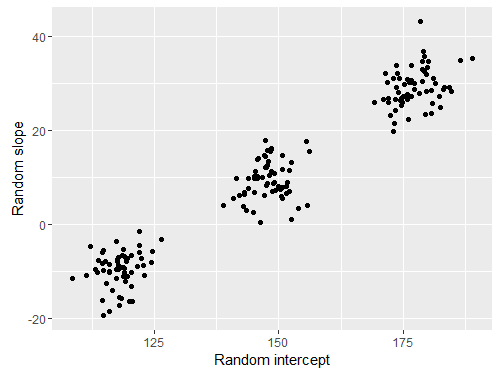
\includegraphics[width=\textwidth]{mainmatter/chapter_5_simulation_study/ds_3wellsep_randplot.png}
        \caption{\label{fig : ds_3wellsep_randplot}Data set 2}
	\end{subfigure}
	\begin{subfigure}[b]{0.4\textwidth}
		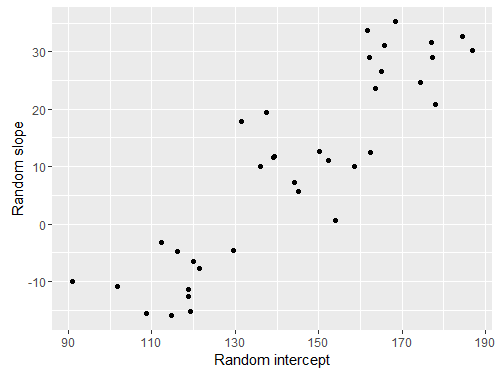
\includegraphics[width=\textwidth]{mainmatter/chapter_5_simulation_study/ds_3wellsep3ppg_randplot.png}
       \caption{\label{fig : ds_3wellsep3ppg_randplot}Data set 3}
	\end{subfigure}    
    
\caption{\label{fig : ds_3comp_3ppgwelsep}Rough estimate $\tilde{\boldsymbol{b}_i}$ for random effects}
\end{figure}

\subsubsection{Data set 5: 3 fused components but less subjects}
\label{subsubsec : ds_3fused_3ppg}
This data is similar to Data set 4 in all regards except for the number of subjects. We generated only 36 subjects in total in this data set. A plot of the rough estimates of random effect values for this data set is shown in figure \ref{fig : ds_3fused3ppg_randplot}.

\subsubsection{Data set 6: 5 well separated components}
\label{subsubsec : ds_5wellsep}
In this data set we simulated the random effects from a mixture distribution which had 5 well separated components. However this time we generated unequal number of subjects for every component. The plot of the rough estimates of random effect values for this data set is shown in figure \ref{fig : ds_5wellsep_randplot}.

\begin{figure}[!htb]
\centering
\begin{subfigure}[b]{0.4\textwidth}
		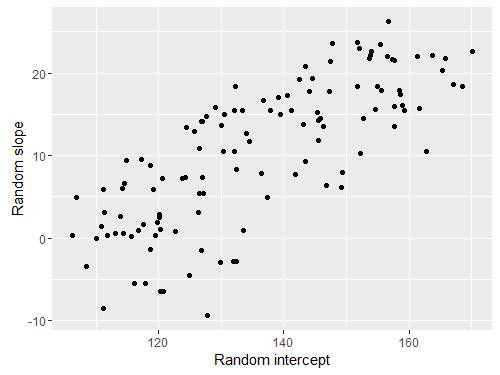
\includegraphics[width=\textwidth]{mainmatter/chapter_5_simulation_study/ds_3fused10ppg_randplot.png}
        \caption{\label{fig : ds_3fused10ppg_randplot}Data set 4}
	\end{subfigure}
	\begin{subfigure}[b]{0.4\textwidth}
		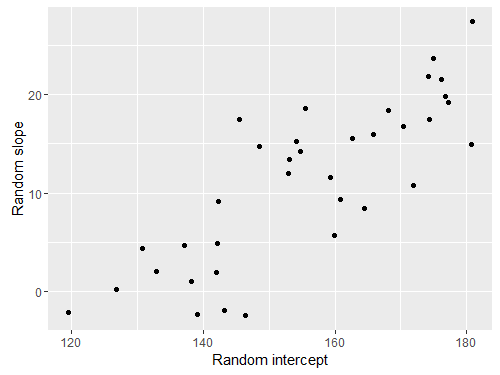
\includegraphics[width=\textwidth]{mainmatter/chapter_5_simulation_study/ds_3fused3ppg_randplot.png}
       \caption{\label{fig : ds_3fused3ppg_randplot}Data set 5}
	\end{subfigure}    
    
\caption{\label{fig : ds_3fused10ppg_3fused3ppg}Rough estimate $\tilde{\boldsymbol{b}_i}$ for random effects}
\end{figure}

\subsubsection{Data set 7: 5 fused components}
\label{subsubsec : ds_5fused}
This data is similar to Data set 6 in all regards except that the number of subjects per component are less, and the components are not so well separated. The plot of the rough estimates of random effect values for this data set is shown in figure \ref{fig : ds_5fused_randplot}.

\begin{figure}[!htb]
\centering
\begin{subfigure}[b]{0.4\textwidth}
		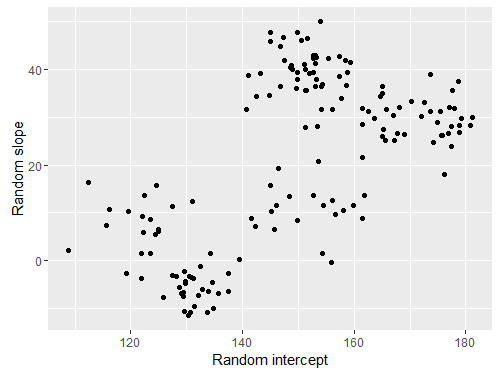
\includegraphics[width=\textwidth]{mainmatter/chapter_5_simulation_study/ds_5wellsep_randplot.png}
        \caption{\label{fig : ds_5wellsep_randplot}Data set 6}
	\end{subfigure}
	\begin{subfigure}[b]{0.4\textwidth}
		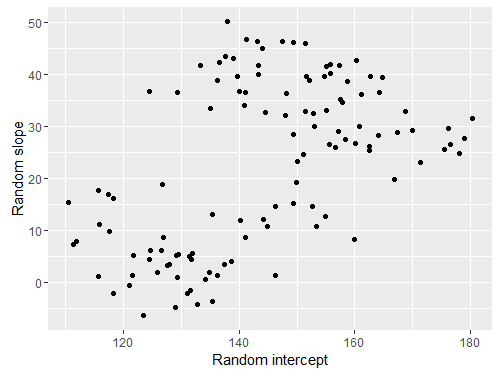
\includegraphics[width=\textwidth]{mainmatter/chapter_5_simulation_study/ds_5fused_randplot.png}
        \caption{\label{fig : ds_5fused_randplot}Data set 7}
	\end{subfigure}
	\caption{Rough estimate $\tilde{\boldsymbol{b}_i}$ for random effects.}
	\label{fig : ds_5wellsep_5fused}    
\end{figure}


\subsection{Running MCMC simulations}
We will first discuss some of the issues we while doing the MCMC simulations. The first was label switching across the chains while calculating Bayes factor using Chib's approximation, i.e. label 1 corresponding to component 1 in one chain and corresponding to some other component in another chain. This gave inconsistent and incorrect estimates for the various calculations we did. Although we dealt with it using the mechanisms given in section \ref{subsec : label_switching_blmm}, it decreased the speed of simulations drastically. To make matters worse we had to employ thinning of 1 per 100 iterations and in some cases 1 per 200 iterations to make sure the resulting chains were not autocorrelated. Since we lacked computational resources required to run long chains we had to be content with chains of length 1300 (after thinning). The following results are based on a single chain and are rounded to the nearest integer.

\subsection{Deviance information criteria}
\label{subsec : dic_simulation_results}
Table \ref{table : ds_simple_dic} shows the values of the various deviance information criteria (section \ref{sec : dic}) applied to data set 1. We can see that $\text{DIC}_1$ gives misleading results with overfitted models. On the other hand the remaining DIC's are relatively stable. We obtained a negative value (-602) for ${\text{p}_\text{D}}_1$ when we fitted 3 components. \citet[pg. 161]{lunn_bugs_2012} noted that this can happen if the posterior is multi modal. As a remedial measure \citet{celeux_deviance_2006} suggested using $\text{DIC}_3$ instead of the other two observed data DIC measures.\\

\begin{table}[!htb]
\centering
\caption{DIC and $\text{p}_\text{D}$ for data set 1. True number of components = 1}
\label{table : ds_simple_dic} 
\begin{tabular}{@{}rrrrrrr@{}}
\toprule
\# Comp Fitted & $\text{DIC}_1$ & $\text{DIC}_2$  & $\text{DIC}_3$  & $\text{DIC}_4$  & $\text{DIC}_5$  & $\text{DIC}_6$  \\ \midrule
1      & 4143 & 4144 & 4143 & 5160 & 4402 & 3483 \\
2      & 4146 & 4147 & 4145 & 5161 & 4403 & 3480 \\
3      & 3536 & 4148 & 4147 & 5163 & 4388 & 3465 \\
4      & 9    & 4151 & 4149 & 5166 & 4407 & 3485 \\ \bottomrule
\end{tabular}

\begin{tabular}{@{}rrrrrrr@{}}
\toprule
\# Comp Fitted & ${\text{p}_\text{D}}_1$ & ${\text{p}_\text{D}}_2$ & ${\text{p}_\text{D}}_3$ & ${\text{p}_\text{D}}_4$ & ${\text{p}_\text{D}}_5$ & ${\text{p}_\text{D}}_6$ \\ \midrule
1      & 9    & 9    & 9    & 903  & 145  & 125  \\
2      & 9    & 10   & 9    & 903  & 145  & 122  \\
3      & -602 & 9    & 8    & 901  & 126  & 107  \\
4      & 9    & 11   & 9    & 903  & 145  & 127  \\ \bottomrule
\end{tabular}
\end{table}

Table \ref{table : ds_3wellsep_dic} shows the values of various DIC we obtained for data set 2. One of the patterns we observe in these results is that the $\text{DIC}_4$ value decreased continuously till the right number of components were fitted, whereas for the overfitted models it either decreased by a bit or remained more or less the same. A similar pattern is observed for $\text{DIC}_5$ and $\text{DIC}_3$. However it seems that they are not as discerning as $\text{DIC}_4$. $\text{DIC}_1$ and $\text{DIC}_6$ do not seem to have any clear pattern. The last pattern we observe is that ${\text{p}_\text{D}}_1$ becomes negative for 4 or more components which is a sign of multi modal posterior as we discussed above.\\

It is important to note that, while a DIC difference of 10 is usually considered good enough to prefer one model over another, this rule may not be as applicable here. The reason is that we have chains of short length and most of the chains with overfitted components also had high autocorrelation despite a thinning of 1 per 200 iterations.\\

\begin{table}[!htb]
\centering
\caption{DIC and $\text{p}_\text{D}$ for data set 2. True number of components = 3}
\label{table : ds_3wellsep_dic} 
\begin{tabular}{@{}rrrrrrr@{}}
\toprule
\# Comp Fitted & $\text{DIC}_1$ & $\text{DIC}_2$  & $\text{DIC}_3$  & $\text{DIC}_4$  & $\text{DIC}_5$  & $\text{DIC}_6$  \\ \midrule
1 & 9966 & 9959 & 9965 & 12921 & 10531 & 7855 \\
2 & 9865 & 9849 & 9864 & 12498 & 10458 & 7860 \\
3 & 9664 & 9665 & 9663 & 11847 & 10244 & 7870 \\
4 & 9516 & 9654 & 9664 & 11834 & 10266 & 7888 \\
5 & 7370 & 9729 & 9666 & 11812 & 10277 & 7870 \\
6 & 9498 & 9661 & 9668 & 11833 & 10242 & 7857 \\ \bottomrule
\end{tabular}

\begin{tabular}{@{}rrrrrrr@{}}
\toprule
\# Comp Fitted & ${\text{p}_\text{D}}_1$ & ${\text{p}_\text{D}}_2$ & ${\text{p}_\text{D}}_3$ & ${\text{p}_\text{D}}_4$ & ${\text{p}_\text{D}}_5$ & ${\text{p}_\text{D}}_6$ \\ \midrule
1 & 9 & 2 & 8 & 2670 & 279 & 269 \\
2 & 15 & -1 & 14 & 2344 & 304 & 272 \\
3 & 21 & 21 & 20 & 1933 & 331 & 282 \\
4 & -125 & 13 & 23 & 1913 & 345 & 298 \\
5 & -2270 & 89 & 26 & 1889 & 355 & 280 \\
6 & -147 & 16 & 23 & 1912 & 321 & 269 \\ \bottomrule
\end{tabular}
\end{table}

Table \ref{table : ds_3wellsep_3ppg_dic} shows the values of the various DIC applied to the data set 3. Firstly we can see that the pattern we observed for ${\text{p}_\text{D}}_1$ in data set 2 is not applicable here. Similar to the results for data set 2, $\text{DIC}_6$ does not reveal any meaningful pattern here. We can also see that the pattern of $\text{DIC}_5$ that we noted above is not applicable here. However for $\text{DIC}_3$ and $\text{DIC}_4$ one can again see that the DIC are decreasing by a large amount till the right number of components are fitted. The magnitudes of all of the the DIC have decreased in comparison to DIC for data set 2 because the sample size for this data set is only 36 subjects compared to 180 subjects in the former.

\begin{table}[!htb]
\centering
\caption{DIC and $\text{p}_\text{D}$ for data set 3. True number of components = 3}
\label{table : ds_3wellsep_3ppg_dic}
\begin{tabular}{@{}rrrrrrr@{}}
\toprule
\# Comp Fitted & $\text{DIC}_1$ & $\text{DIC}_2$  & $\text{DIC}_3$  & $\text{DIC}_4$  & $\text{DIC}_5$  & $\text{DIC}_6$  \\ \midrule
1 & 2013 & 2012 & 2012 & 2611 & 2118 & 1570 \\
2 & 1989 & 1949 & 1987 & 2497 & 2013 & 1562 \\
3 & 1942 & 1942 & 1940 & 2339 & 2039 & 1571 \\
4 & 1943 & 1944 & 1942 & 2342 & 2034 & 1559 \\
5 & 1936 & 1940 & 1944 & 2344 & 2049 & 1580 \\
6 & 1695 & 1948 & 1945 & 2344 & 2053 & 1579 \\ \bottomrule
\end{tabular}

\begin{tabular}{@{}rrrrrrr@{}}
\toprule
\# Comp Fitted & ${\text{p}_\text{D}}_1$ & ${\text{p}_\text{D}}_2$ & ${\text{p}_\text{D}}_3$ & ${\text{p}_\text{D}}_4$ & ${\text{p}_\text{D}}_5$ & ${\text{p}_\text{D}}_6$ \\ \midrule
1 & 8 & 7 & 7 & 545 & 52 & 45 \\
2 & 14 & -26 & 12 & 465 & -20 & 35 \\
3 & 17 & 17 & 15 & 370 & 70 & 46 \\
4 & 16 & 17 & 15 & 370 & 62 & 34 \\
5 & 8 & 11 & 15 & 370 & 75 & 56 \\
6 & -235 & 17 & 15 & 368 & 77 & 53 \\ \bottomrule
\end{tabular}
\end{table}

Table \ref{table : ds_3fused_10ppg_dic} shows the results of applying various DIC to data set 4. So far we have observed that $\text{DIC}_3$ and $\text{DIC}_4$ can be used to detect the right number of components. Since the components in this data set are fused, and the subjects count is moderately high, the following results are interesting to analyze. We can see that $\text{DIC}_4$ still follows the pattern we have discussed so far, but with $\text{DIC}_3$ and $\text{DIC}_5$ it is a bit difficult to justify. To further validate the patterns we observed so far, we decided to decrease the number of subjects to 36.\\
 
\begin{table}[!htb]
\centering
\caption{DIC and $\text{p}_\text{D}$ for data set 4}
\label{table : ds_3fused_10ppg_dic}
\begin{tabular}{@{}rrrrrrr@{}}
\toprule
\# Comp Fitted & $\text{DIC}_1$ & $\text{DIC}_2$  & $\text{DIC}_3$  & $\text{DIC}_4$  & $\text{DIC}_5$  & $\text{DIC}_6$  \\ \midrule
1 & 6568 & 6566 & 6566 & 8454 & 6899 & 5197 \\
2 & 6531 & 6523 & 6530 & 8263 & 6946 & 5253 \\
3 & 6497 & 6492 & 6497 & 8017 & 6898 & 5263 \\
4 & 6347 & 6480 & 6488 & 7955 & 6898 & 5253 \\
5 & 6321 & 6463 & 6485 & 7932 & 6743 & 5259 \\
6 & 6382 & 6329 & 6489 & 7948 & 6611 & 5259 \\ \bottomrule
\end{tabular}

\begin{tabular}{@{}rrrrrrr@{}}
\toprule
\# Comp Fitted & ${\text{p}_\text{D}}_1$ & ${\text{p}_\text{D}}_2$ & ${\text{p}_\text{D}}_3$ & ${\text{p}_\text{D}}_4$ & ${\text{p}_\text{D}}_5$ & ${\text{p}_\text{D}}_6$ \\ \midrule
1 & 9 & 8 & 8 & 1694 & 139 & 127 \\
2 & 14 & 7 & 13 & 1527 & 210 & 182 \\
3 & 20 & 14 & 19 & 1341 & 222 & 187 \\
4 & -115 & 17 & 26 & 1287 & 230 & 181 \\
5 & -138 & 4 & 26 & 1265 & 76 & 187 \\
6 & -81 & -134 & 26 & 1275 & -62 & 185 \\ \bottomrule
\end{tabular}
\end{table}

Table \ref{table : ds_3fused_3ppg_dic} shows the results of DIC for data set 5. At first glance one can see that the pattern we saw so far for $\text{DIC}_4$ doesn't exist anymore. However, the catch here is that these results are based on a dirichlet prior $\text{Dir}(1, 1, ..., 1)$ for the weight distribution. When we fitted 2 or more components we found that the MCMC chains had not converged with this prior. Given the fused data set, even if one fits 2 components there is a risk of unidentifiability due to empty components.\\

We changed the prior for weight distribution to $\text{Dir}(3, 3, ..., 3)$ and fitted models with 2, 3 and 4 components for the mixture. With 2 components we found $\text{DIC}_4 = 2441 ({\text{p}_\text{D}}_4 = 461)$ and $\text{DIC}_3 = 1937 ({\text{p}_\text{D}}_3 = 14)$. For 3 components we obtained $\text{DIC}_4$ = 2352 and for 4 components we obtained $\text{DIC}_4 = 2346$. For 4 components $\text{DIC}_3 = 1925$. In light of these results one can still justify the pattern we have observed for $\text{DIC}_4$ so far but not for $\text{DIC}_3$. An interesting result from this exercise was that the choice of $\text{Dir}(1, 1, ..., 1)$ prior is prone to severe underfitting.

\begin{table}[!htb]
\centering
\caption{DIC and $\text{p}_\text{D}$ for data set 5.}
\label{table : ds_3fused_3ppg_dic}
\begin{tabular}{@{}rrrrrrr@{}}
\toprule
\# Comp Fitted & $\text{DIC}_1$ & $\text{DIC}_2$  & $\text{DIC}_3$  & $\text{DIC}_4$  & $\text{DIC}_5$  & $\text{DIC}_6$  \\ \midrule
1 & 1944 & 1943 & 1943 & 2500 & 1879 & 1364 \\
2 & 1936 & 1941 & 1945 & 2487 & 1919 & 1408 \\
3 & 1886 & -3353 & 1944 & 2453 & -$\infty$ & 1525 \\
4 & 1892 & 1904 & 1944 & 2439 & 1851 & 1389 \\
5 & 1902 & 1840 & 1942 & 2418 & 704 & 336 \\
6 & 1883 & 1919 & 1933 & 2371 & 2023 & 1538 \\ \bottomrule
\end{tabular}

\begin{tabular}{@{}rrrrrrr@{}}
\toprule
\# Comp Fitted & ${\text{p}_\text{D}}_1$ & ${\text{p}_\text{D}}_2$ & ${\text{p}_\text{D}}_3$ & ${\text{p}_\text{D}}_4$ & ${\text{p}_\text{D}}_5$ & ${\text{p}_\text{D}}_6$ \\ \midrule
1 & 9 & 7 & 7 & 510 & -110 & -119 \\
2 & 2 & 7 & 11 & 500 & -68 & -73 \\
3 & -42 & -5281 & 16 & 470 & -$\infty$ & 41 \\
4 & -34 & -22 & 18 & 459 & -130 & -93 \\
5 & -21 & -83 & 19 & 442 & -1272 & -1146 \\
6 & -31 & 5 & 19 & 407 & 59 & 55 \\ \bottomrule
\end{tabular}
\end{table}

Table \ref{table : ds_5wellsep_dic} shows the results of applying DIC to the various models fitted for data set 6. The pattern of $\text{DIC}_4$ decreasing by a large margin till the right number of components (5 in this case) are fitted is visible here as well. What is more interesting is that $\text{DIC}_3$ also seem to work well in this case. This is an indication that $\text{DIC}_3$ can used to select the correct model if the components are well separated.\\

\begin{table}[!htb]
\centering
\caption{DIC and $\text{p}_\text{D}$ for data set 6}
\label{table : ds_5wellsep_dic}
\begin{tabular}{@{}rrrrrrr@{}}
\toprule
\# Comp Fitted & $\text{DIC}_1$ & $\text{DIC}_2$  & $\text{DIC}_3$  & $\text{DIC}_4$  & $\text{DIC}_5$  & $\text{DIC}_6$  \\ \midrule
1 & 8982 & 8981 & 8980 & 11847 & 9251 & 6655 \\
2 & 8829 & 8827 & 8827 & 11327 & 9293 & 6838 \\
3 & 8745 & 8742 & 8744 & 11036 & 9251 & 6895 \\
4 & 8669 & 8672 & 8677 & 10737 & 9208 & 6925 \\
5 & 8649 & 8643 & 8648 & 10601 & 9165 & 6909 \\
6 & 8096 & 8697 & 8650 & 10594 & 9183 & 6923 \\
7 & 7770 & 8364 & 8651 & 10593 & 7613 & 6919 \\
8 & 8196 & 8640 & 8653 & 10597 & 9143 & 6927 \\ \bottomrule
\end{tabular}

\begin{tabular}{@{}rrrrrrr@{}}
\toprule
\# Comp Fitted & ${\text{p}_\text{D}}_1$ & ${\text{p}_\text{D}}_2$ & ${\text{p}_\text{D}}_3$ & ${\text{p}_\text{D}}_4$ & ${\text{p}_\text{D}}_5$ & ${\text{p}_\text{D}}_6$ \\ \midrule
1 & 9 & 9 & 7 & 2591 & -5 & -14 \\
2 & 14 & 13 & 12 & 2224 & 190 & 169 \\
3 & 20 & 16 & 19 & 2035 & 250 & 223 \\
4 & 19 & 23 & 27 & 1824 & 296 & 251 \\
5 & 31 & 26 & 30 & 1725 & 289 & 232 \\
6 & -520 & 81 & 33 & 1711 & 300 & 246 \\
7 & -848 & -254 & 34 & 1706 & -1274 & 244 \\
8 & -424 & 19 & 33 & 1711 & 257 & 248 \\ \bottomrule
\end{tabular}
\end{table}

\begin{table}[!htb]
\centering
\caption{DIC and $\text{p}_\text{D}$ for data set 7}
\label{table : ds_5fused_dic}
\begin{tabular}{@{}rrrrrrr@{}}
\toprule
\# Comp Fitted & $\text{DIC}_1$ & $\text{DIC}_2$  & $\text{DIC}_3$  & $\text{DIC}_4$  & $\text{DIC}_5$  & $\text{DIC}_6$  \\ \midrule
1 & 6708 & 6707 & 6706 & 8819 & 6977 & 5071 \\
2 & 6606 & 6605 & 6604 & 8443 & 6946 & 5135 \\
3 & 6539 & 6538 & 6537 & 8178 & 6944 & 5204 \\
4 & 6506 & 6514 & 6521 & 8078 & 6915 & 5196 \\
5 & 6505 & 6500 & 6508 & 7984 & 6896 & 5202 \\
6 & 6465 & 6501 & 6510 & 7988 & 6895 & 5196 \\
7 & 6200 & 6500 & 6512 & 7989 & 6883 & 5190 \\
8 & 6448 & 6498 & 6516 & 7995 & 6901 & 5196 \\ \bottomrule
\end{tabular}

\begin{tabular}{@{}rrrrrrr@{}}
\toprule
\# Comp Fitted & ${\text{p}_\text{D}}_1$ & ${\text{p}_\text{D}}_2$ & ${\text{p}_\text{D}}_3$ & ${\text{p}_\text{D}}_4$ & ${\text{p}_\text{D}}_5$ & ${\text{p}_\text{D}}_6$ \\ \midrule
1 & 9 & 8 & 7 & 1903 & 61 & 53 \\
2 & 15 & 14 & 13 & 1636 & 139 & 120 \\
3 & 21 & 20 & 19 & 1456 & 221 & 185 \\
4 & 12 & 20 & 26 & 1381 & 218 & 176 \\
5 & 26 & 22 & 29 & 1308 & 220 & 182 \\
6 & -14 & 21 & 30 & 1307 & 214 & 176 \\
7 & -282 & 18 & 30 & 1305 & 198 & 168 \\
8 & -36 & 14 & 32 & 1307 & 213 & 175 \\ \bottomrule
\end{tabular}
\end{table}

Table \ref{table : ds_5fused_dic} shows the results of applying DIC to the various models fitted for data set 7. Based on figure \ref{fig : ds_5fused_randplot} one might only choose 3 components in this mixture. The pattern of $\text{DIC}_4$ decreasing by a large margin till the right number of components (5 in this case) are fitted is visible here as well. Although again the pattern for $\text{DIC}_3$ is a bit difficult to justify despite the large sample size.

\subsection{Marginal likelihood}
\label{subsec : marginal_likelihood_simulation}
We implemented Chib's approximation mentioned in section \ref{sec : marginal_likelihood}. Table \ref{table : marginal_likelihood_results} shows the results of $\log{\hat{m}(\boldsymbol{y})}$ for the various models we fitted to data set 1 to data set 7. One can see that there is no obvious pattern visible in these results to conclude the efficacy of Bayes factor in selection of a model. For e.g. in case of data set 6 we had 5 well separated components in the mixture distribution of random effects. When we fitted 1,2,3,4 and 5 components to this data set we had MCMC chains with good convergence and no multi-modality was observed for the posteriors. However we can see that marginal likelihood preferred fitting 1 component over higher number of components. For data set 3 where we had 3 well separated components but only 36 subjects in total, we can observe that marginal likelihood is almost the same for 1,2 and 3 components, making it difficult to make a choice for the number of components.

\begin{table}[!htb]
\centering
\caption{$\log{\hat{m}(\boldsymbol{y})}$ for data set 1}
\label{table : marginal_likelihood_results} 
\begin{tabular}{rrrrrrrrr}
\toprule
Fitted & 1 Comp & 2 Comp & 3 Comp & 4 Comp & 5 Comp & 6 Comp & 7 Comp & 8 Comp \\\midrule
Data set 1 & -2120 & -2128 & -2139 & -2142 &  &  &  &  \\
Data set 2 & -5019 & -4989 & -4937 & -4925 & -4938 & $\infty$ &  &  \\
Data set 3 & -1038 & -1044 & -1042 & -645 & -1003 & $\infty$ &  &  \\
Data set 4 & -3317 & -3318 & -3322 & -3332 & -3348 & $\infty$ &  &  \\
Data set 5 & -1001 & -1016 & -1032 & -1041 & -1058 & $\infty$ &  &  \\
Data set 6 & -4545 & -4492 & -4477 & -4467 & -4473 & $\infty$ & -4498 & -3985 \\
Data set 7 & -3397 & -3379 & -3373 & -3380 & -2749 & $\infty$ & $\infty$ & -3416 \\ \bottomrule
\end{tabular}
\end{table}

\subsection{Posterior predictive check (PPC)}
\label{subsec : ppc_simulation}
We implemented the PPC outlined in section \ref{sec : ppc}. Since the PPC we are using is designed to detect non identifiability due to empty components, it works irrespective of the size of the data set or how well separated the components are. Thus we found the results of PPC to be consistent across the various data sets. Because of this reason, we will only discuss the results of fitting various number of components in data set 6. Figure \ref{fig : ppc_5wellsep8comp} to \ref{fig : ppc_5wellsep1comp} show the distribution of the test statistic \ref{eq : ppc_test_statistic} for the various models we fitted to data 6. It can be seen that the distribution is positively skewed whenever overfitting is present. On the other hand the distribution of the test statistic is more or less the same in cases of underfitting. It is to be noted that this is despite the fact that we used a mixed predictive approach.\\

\begin{figure}[!htb]
\centering
\begin{subfigure}[b]{0.4\textwidth}
		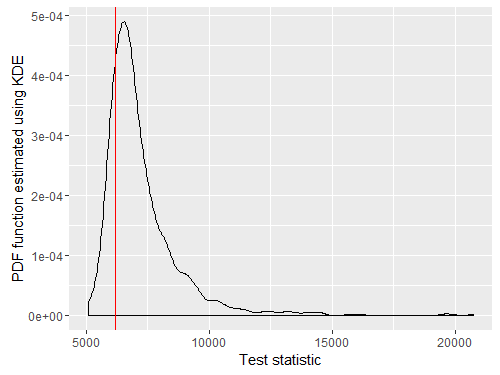
\includegraphics[width=\textwidth]{mainmatter/chapter_5_simulation_study/ppc_5wellsep8comp.png}
        \caption{\label{fig : ppc_5wellsep8comp}8 components fitted for data set 6}
	\end{subfigure}
	\begin{subfigure}[b]{0.4\textwidth}
		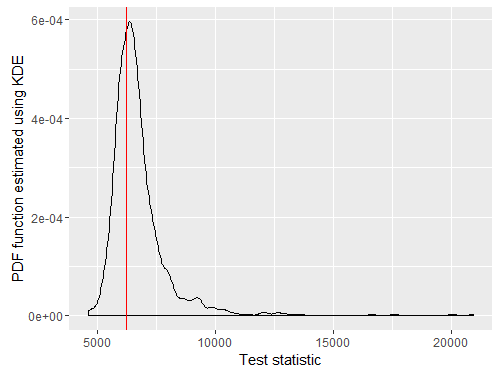
\includegraphics[width=\textwidth]{mainmatter/chapter_5_simulation_study/ppc_5wellsep7comp.png}
          \caption{\label{fig : ppc_5wellsep7comp}7 components fitted for data set 6}
	\end{subfigure}
	\begin{subfigure}[b]{0.4\textwidth}
		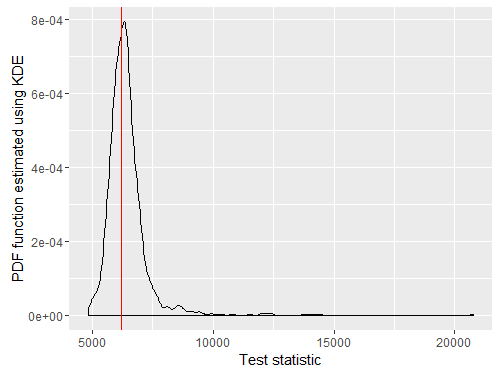
\includegraphics[width=\textwidth]{mainmatter/chapter_5_simulation_study/ppc_5wellsep6comp.png}
          \caption{\label{fig : ppc_5wellsep6comp}6 components fitted for data set 6}
	\end{subfigure}
	\begin{subfigure}[b]{0.4\textwidth}
		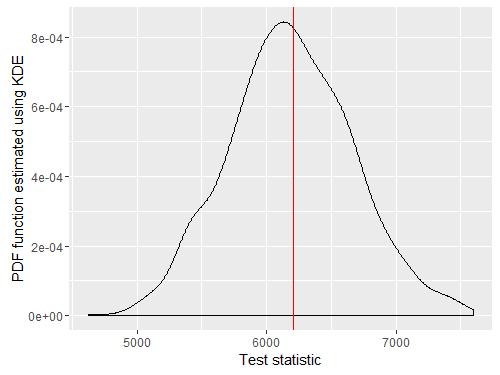
\includegraphics[width=\textwidth]{mainmatter/chapter_5_simulation_study/ppc_5wellsep5comp.png}
          \caption{\label{fig : ppc_5wellsep5comp}5 components fitted for data set 6}
	\end{subfigure}
	\begin{subfigure}[b]{0.4\textwidth}
		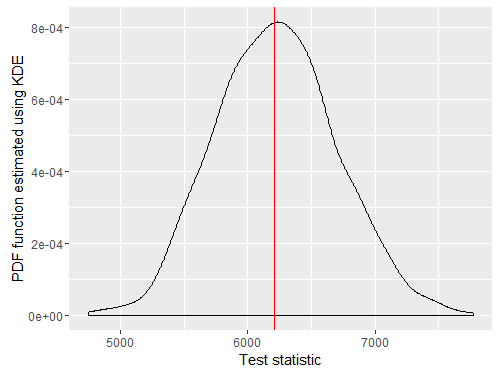
\includegraphics[width=\textwidth]{mainmatter/chapter_5_simulation_study/ppc_5wellsep4comp.png}
          \caption{\label{fig : ppc_5wellsep4comp}4 components fitted for data set 6}
	\end{subfigure}
	\begin{subfigure}[b]{0.4\textwidth}
		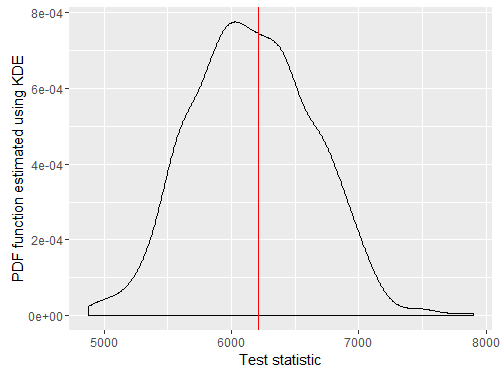
\includegraphics[width=\textwidth]{mainmatter/chapter_5_simulation_study/ppc_5wellsep3comp.png}
          \caption{\label{fig : ppc_5wellsep3comp}3 components fitted for data set 6}
	\end{subfigure}
	\begin{subfigure}[b]{0.4\textwidth}
		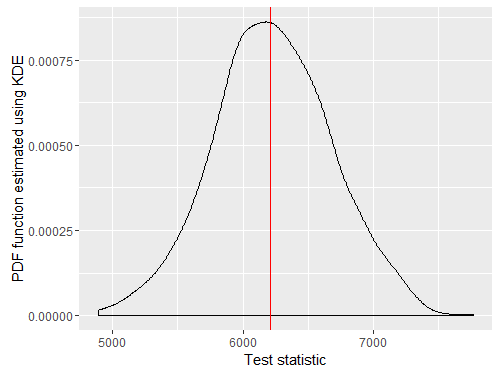
\includegraphics[width=\textwidth]{mainmatter/chapter_5_simulation_study/ppc_5wellsep2comp.png}
          \caption{\label{fig : ppc_5wellsep2comp}2 components fitted for data set 6}
	\end{subfigure}
	\begin{subfigure}[b]{0.4\textwidth}
		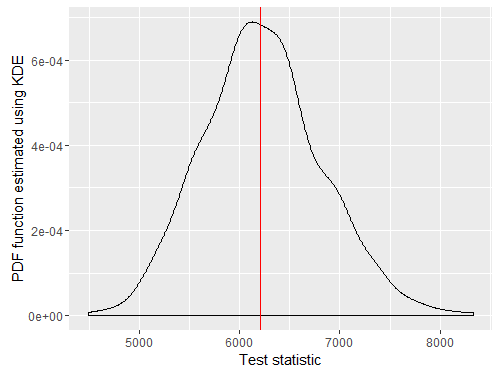
\includegraphics[width=\textwidth]{mainmatter/chapter_5_simulation_study/ppc_5wellsep1comp.png}
          \caption{\label{fig : ppc_5wellsep1comp}1 component fitted for data set 6}
	\end{subfigure}
	\caption{PDF function of $T(\boldsymbol{\tilde{r}})$ estimated using KDE. The red line shows the value of the test statistic $T(\boldsymbol{r})$ based on the observed data.}
	\label{fig : ppc_5wellsepcomp}    
\end{figure}

One can observe a more severe impact of overfitting if they use independent inverse gamma priors for the variance components of $G_k$ and uniform prior $U(-1,1)$ for correlation. To show the resulting distribution of the test statistic, we had to log transform it as otherwise the values were too large to be plotted in a single graph. We took the case of data set 2 and overfitted the mixture of random effects by using 4 components in the mixture. One can see that the corresponding test statistic inflates by a large margin as we described in section \ref{sec : ppc}. Interestingly when we fit the right number of components the test statistic is not inflated, but we can still see that the model is not well fitting. We further checked our posteriors for variance covariance matrices and found them to be underestimating the original variance covariance of the random effects from the simulated data set. This proves that the test statistic can be used to detect bad fitting models, however differentiating among models with less number of components may not be possible.

\begin{figure}[!h]
	\centering
	\begin{subfigure}[b]{0.4\textwidth}
		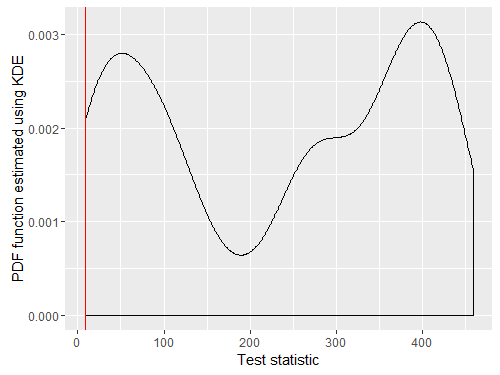
\includegraphics[width=\textwidth]{mainmatter/chapter_5_simulation_study/indpGammaPrior_ppc_3wellsep4comp.png}
        \caption{\label{fig : ppc_3wellsep3comp_indp_gammaprior}4 components fitted for data set 2. log scale is used.}
	\end{subfigure}
	\begin{subfigure}[b]{0.4\textwidth}
		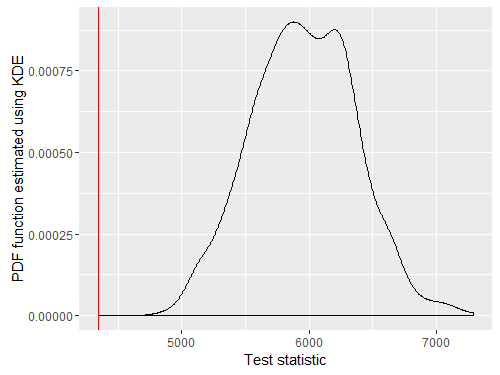
\includegraphics[width=\textwidth]{mainmatter/chapter_5_simulation_study/indpGammaPrior_ppc_3wellsep3comp.png}
        \caption{\label{fig : ppc_3wellsep3comp_indp_gammaprior}3 components fitted for data set 2}
	\end{subfigure}
	\caption{PDF function of $T(\boldsymbol{\tilde{r}})$ estimated using KDE. The red line shows the value of the test statistic $T(\boldsymbol{r})$ based on the observed data. Indepdent gamma priors for precision and uniform prior for correlation is used.}
	\label{fig : ppc_3wellsep4comp_indp_gammaprior}
\end{figure}